%!TEX TS-program = xelatex
\documentclass{EdipyLabs} % Custom class provided for EDIPY labs, by Christos Dalamagkas (cdalamagkas@gmail.com)
\SetLabNumber{0}
\SetLabTitle{Παρουσίαση εργαστηριακού εξοπλισμού ΕΔΙΠΥ}
\SetAuthor{Χρήστος Δαλαμάγκας}
\SetLabDescription{Εξοικείωση με τον εξοπλισμό του εργαστηρίου, οπτική αναγνώριση μιας δικτυακής συσκευής και των διεπαφών της.}
\SetLabPrerequisites{Βασική ορολογία Δικτύων Υπολογιστών.}

\lhead{\footnotesize \LabTitle}

\begin{document}
	
\begin{titlepage}
	\centering % Center everything on the page
	
\includegraphics[scale=0.4]{icte-uowm.pdf}\\[1cm]
	
	%	HEADING SECTIONS
	\textsc{\Huge Πανεπιστημιο Δυτικησ Μακεδονιασ}\\[0.5cm] % University name
	\textsc{\Large Τμημα Μηχανικων Πληροφορικησ και Τηλεπικοινωνιων}\\[0.5cm] % Department name
	\large{Εργαστήριο Δικτύων και Προηγμένων Υπηρεσιών}\\[0.5cm] % course title
	
	%	TITLE SECTION
	\rule{\linewidth}{0.5mm}\\[0.25cm]
	{\LARGE\bfseries \LabTitle}\\ % Lab title
	\rule{\linewidth}{0.5mm}\\[1.25cm]
	
	%	AUTHOR SECTION
	%\begin{minipage}{0.85\textwidth}
	%	\begin{flushleft}
	%		\textit{Επιμέλεια:}\\[0.125cm]
	%		\Author\\
	%	\end{flushleft}
	%\end{minipage}
	
	\vfill % Fill the rest of the page with whitespace
	
	%	DATE SECTION
	{\large Κοζάνη, \today} 
	
\end{titlepage}

\section*{Περιγραφή}
\textbf{Λέξεις κλειδιά}: \LabDescription \par
\textbf{Προαπαιτούμενες γνώσεις}: \LabPrerequisites\par
\renewcommand{\baselinestretch}{\dnormalspacing}
\small
\titlespacing{\section}{0cm}{1cm}{0cm}
\tableofcontents
\titlespacing{\section}{0cm}{1cm}{0.25cm}	
\listoffigures
\titlespacing{\section}{0cm}{0.25cm}{-0.125cm}
\titlespacing{\subsection}{0cm}{0.25cm}{-0.125cm}
\titlespacing{\subsubsection}{0cm}{0.25cm}{-0.125cm}
\renewcommand{\baselinestretch}{\dnormalspacing}\normalsize
\newpage

\section{Μεταγωγείς}
Οι μεταγωγείς (switches) αποτελούν δικτυακές συσκευές που επεξεργάζονται δεδομένα στο επίπεδο ζεύξης δεδομένων του OSI και εξυπηρετούν στην μεταγωγή πλαισίων. Οι μεταγωγείς αποκαλούνται και «γέφυρες πολλών θυρών», διότι οι θύρες τους λειτουργούν ως «γέφυρες» (bridge), δηλαδή φέρνουν στο ίδιο δίκτυο πολλαπλά φυσικά μέσα μετάδοσης.

Ο εξοπλισμός του εργαστηρίου αποτελείται από συσκευές Cisco, και συγκεκριμένα, από τη δημοφιλή σειρά Catalyst 2960. Οι συσκευές που χρησιμοποιούνται για τη διεξαγωγή εργαστηριακών ασκήσεων διαθέτουν το λειτουργικό σύστημα Cisco IOS έκδοσης 15.
\subsection{Cisco Catalyst 2960-X}
\begin{figure}[H]
	\centering
	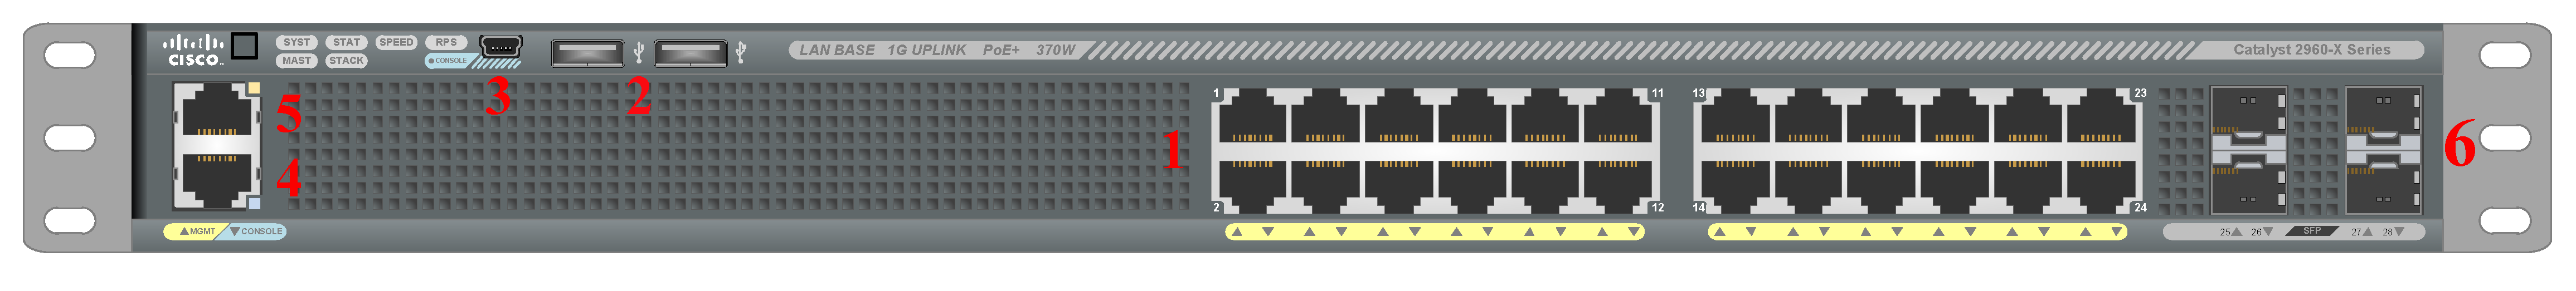
\includegraphics[width=\linewidth]{c2960x.pdf}
	\caption{Ο μεταγωγέας Cisco Catalyst 2960-X}\label{fig:c2960x}
\end{figure}

Οι 2 μεταγωγείς Cisco Catalyst 2960-X του εργαστηρίου (πλήρης ονομασία: WS-C2960X-24PS-L) αποτελούνται από τις εξής διεπαφές:
\begin{enumerate}
	\item x24 θύρες Gigabit Ethernet (10/100/1000 Mbps) με υποστήριξη PoE+
	\item x2 θύρες USB τύπου A
	\item x1 θύρα κονσόλας USB mini-B
	\item x1 θύρα κονσόλας RJ-45
	\item x1 θύρα MGMT Fast Ethernet
	\item x4 θύρες SFP ανόδου με υποστήριξη Gigabit
\end{enumerate}

\subsubsection*{Διαδικασία ενεργοποίησης μηχανήματος}
Για να ενεργοποιήσετε τον μεταγωγέα, συνδέστε το καλώδιο τροφοδοτικού στην κατάλληλη θύρα, στην πίσω όψη της συσκευής. 

Οι μεταγωγείς ενεργοποιούνται αυτόματα, με την παροχή ρεύματος. 

\subsubsection*{Διαδικασία απενεργοποίησης μηχανήματος}
Για να απενεργοποιήσετε τον μεταγωγέα, απλώς αποσυνδέστε το καλώδιο τροφοδοσίας. 

Οι μεταγωγείς δεν διαθέτουν διακόπτη απενεργοποίησης. 

\newpage
\subsection{Cisco Catalyst 2960-SF}
\begin{figure}[H]
	\centering
	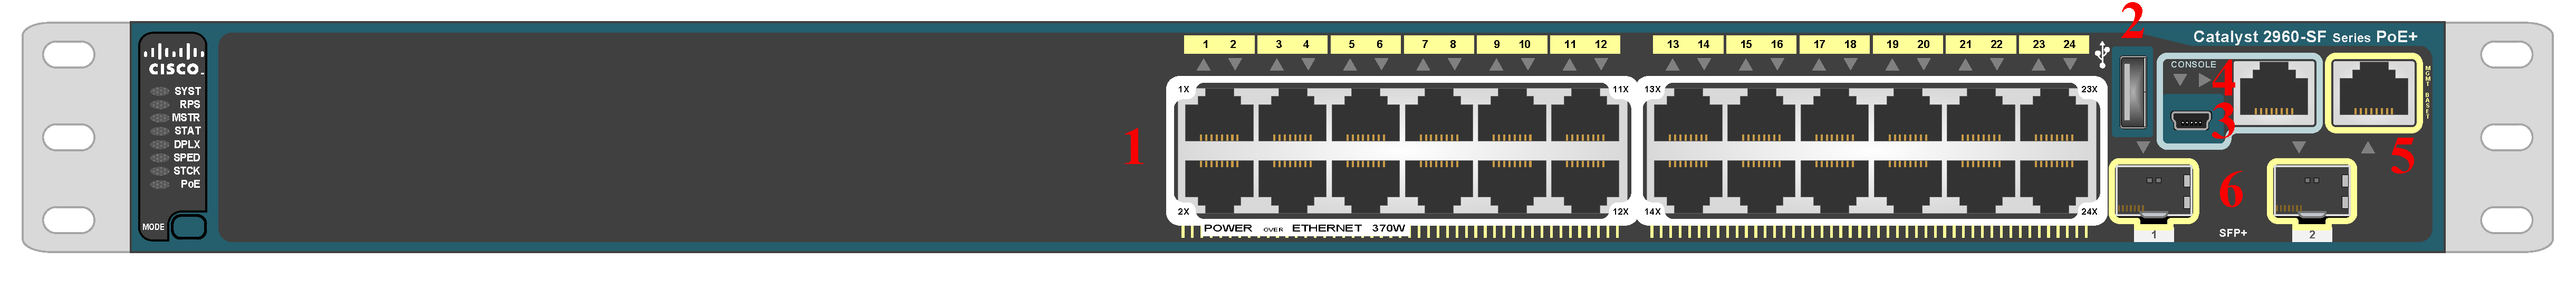
\includegraphics[width=\linewidth]{c2960sf.pdf}
	\caption{Ο μεταγωγέας Cisco Catalyst 2960-SF}\label{fig:c2960sf}
\end{figure}
Οι δυο μεταγωγείς Cisco Catalyst 2960-SF (πλήρης ονομασία: Cisco Catalyst 2960S-24PD-L) αποτελούνται από τις εξής διεπαφές:
\begin{enumerate}
	\item x24 θύρες Fast Ethernet (10/100 Mbps) με υποστήριξη Power over Ethernet + (PoE+)
	\item x1 θύρα USB τύπου A
	\item x1 θύρα κονσόλας USB τύπου mini-B
	\item x1 θύρα κονσόλας RJ-45
	\item x1 θύρα MGMT (Management) Fast Ethernet
	\item x2 θύρες Small Form-Factor Pluggable (SFP) ανόδου με υποστήριξη Gigabit
\end{enumerate}

\subsubsection*{Διαδικασία ενεργοποίησης και απενεργοποίησης μηχανήματος}
Για να ενεργοποιήσετε τον μεταγωγέα, συνδέστε το καλώδιο τροφοδοτικού στην κατάλληλη θύρα, στην πίσω όψη της συσκευής. Η απενεργοποίηση γίνεται αφαιρώντας το ίδιο καλώδιο

Οι μεταγωγείς συνήθως ενεργοποιούνται αυτόματα, με την παροχή ρεύματος και δε διαθέτουν διακόπτη τροφοδοσίας.

\newpage

\section{Δρομολογητές}

Οι δρομολογητές (routers) αποτελούν δικτυακές συσκευές στρώματος δικτύου του OSI, οι οποίες προωθούν πακέτα μεταξύ διαφορετικών δικτύων. Σε αντίθεση με τους μεταγωγείς, οι οποίοι κατά κανόνα αφορούν την επικοινωνία μεταξύ υπολογιστών στο ίδιο δίκτυο, οι δρομολογητές επιτρέπουν την επικοινωνία μεταξύ διαφορετικών δικτύων IP, τα οποία μάλιστα ανήκουν σε διαφορετικούς τομείς ευρυεκπομπής (broadcast domains). Επισημαίνεται ότι κάθε διεπαφή Etnernet ενός δρομολογητή προορίζεται για διαφορετικό δίκτυο IP, σε αντίθεση με τις θύρες ενός μεταγωγέα, οι οποίες είναι γεφυρωμένες, δηλαδή ανήκουν στο ίδιο δίκτυο/τομέα ευρυεκπομπής. 

Το εργαστήριο διαθέτει δρομολογητές από τις εταιρίες Cisco και MikroTik, με την κάθε εταιρεία να εξοπλίζει τις συσκευές της με διαφορετικό λειτουργικό σύστημα.

\subsection{Cisco 2921 Integrated Services Router}
\begin{figure}[H]
	\centering
	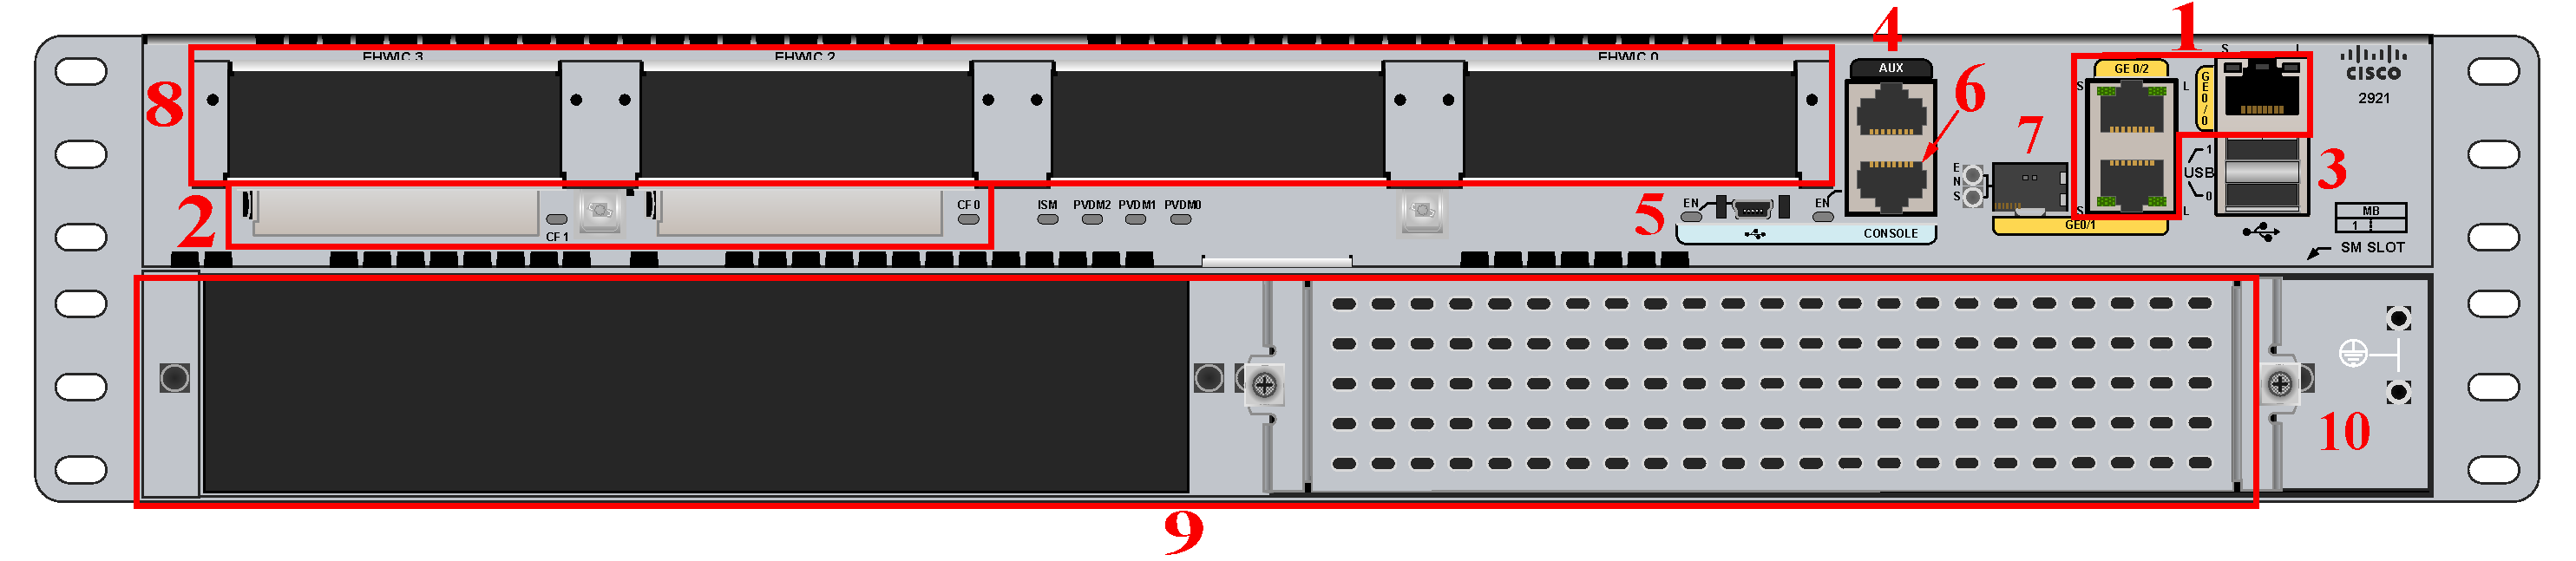
\includegraphics[width=\linewidth]{c2921.pdf}
	\caption{Ο δρομολογητής Cisco 2921 Integrated Services}\label{fig:c2921}
\end{figure}
Οι δρομολογητές Cisco 2921 Integrated Services (ISR) αποτελούνται από τις εξής διεπαφές:
\begin{enumerate}
\item x3 θύρες Gigabit Ethernet (10/100/1000 Mbps)
\item x2 υποδοχές αποθήκευσης CompactFlash
\item x2 θύρες USB τύπου A
\item x1 θύρα Auxiliary (AUX) RJ-45
\item x1 Θύρα κονσόλας USB mini-B
\item x1 Θύρα κονσόλας RJ-45
\item x1 θύρα SFP
\item x4 υποδοχές Cisco Enhanced High-Speed WAN Interface Cards (EHWIC)
\item x2 υποδοχές μονάδων υπηρεσιών (service module slots)
\item Γείωση
\end{enumerate} 
Οι δρομολογητές Cisco υποστηρίζουν πολλές ακόμη υπηρεσίες, που επεκτείνονται σε υψηλότερα επίπεδα του OSI και εστιάζουν στην ασφάλεια, όπως ιδιωτικό εικονικό δίκτυο (VPN), τείχος ασφαλείας (firewall) και σύστημα πρόληψης παρείσδυσης (intrusion prevension system - IPS)

Οι δρομολογητές Cisco εκτελούν το λειτουργικό σύστημα Cisco IOS έκδοσης 15.0.

\subsubsection*{Διαδικασία ενεργοποίησης και απενεργοποίησης μηχανήματος}
Για να ενεργοποιήσετε ή να απενεργοποιήσετε τον δρομολογητή, πατήστε τον διακόπτη τροφοδοσίας που βρίσκεται στην πίσω όψη της συσκευής. 

\newpage

\subsection{MikroTik CCR-1009-8G-1S-1S+}
\begin{figure}[H]
	\centering
	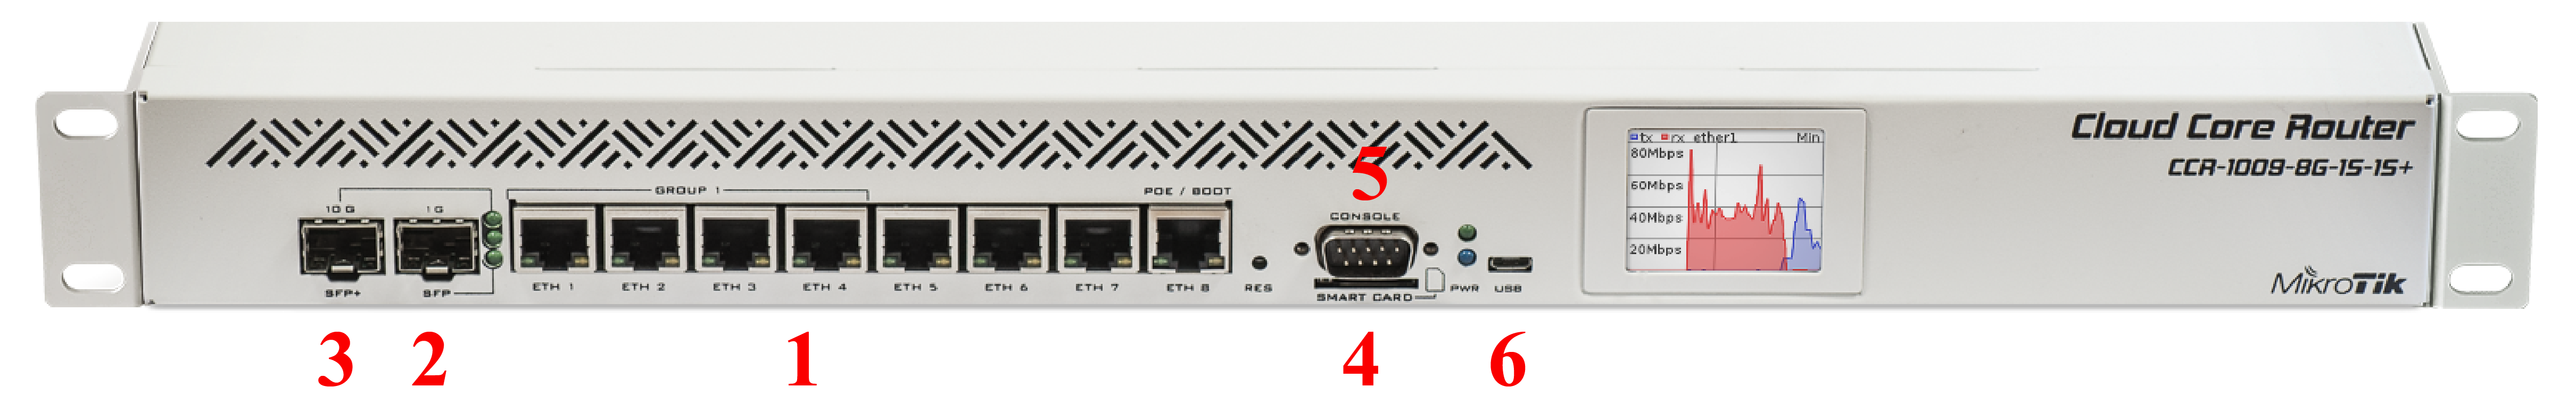
\includegraphics[width=\linewidth]{ccr}
	\caption{Ο δρομολογητής MikroTik CCR-1009-8G-1S-1S+}\label{fig:ccr}
\end{figure}
Ο δρομολογητής MikroTik CCR-1009-8G-1S-1S+ αποτελείται από τις εξής διεπαφές:
\begin{enumerate}
	\item x8 θύρες Gigabit Ethernet, με τις θύρες 1-4 να είναι switch ports, δηλαδή ανήκουν σε μεταγωγέα που βρίσκεται στο εσωτερικό του δρομολογητή. 
	\item x1 θύρα SFP
	\item x1 θύρα SFP+
	\item x1 υποδοχή Smart Card
	\item x1 θύρα κονσόλας σειριακή DB9 RS232C
	\item x1 θύρα micro USB
\end{enumerate} 

Οι δρομολογητές MiktroTik εκτελούν το λειτουργικό σύστημα RouterOS.

Σε αντίθεση με το Cisco IOS, το RouterOS είναι ελεύθερα διαθέσιμο για λήψη από το διαδίκτυο και μπορεί να εγκατασταθεί όχι μόνο σε συσκευές MikroTik αλλά σε οποιονδήποτε υπολογιστή ή εικονική μηχανή ως αυτόνομο λειτουργικό σύστημα, μετατρέποντας ένα οποιοδήποτε μηχάνημα σε δρομολογητή με όλες τις βασικές λειτουργίες.

\subsubsection*{Διαδικασία ενεργοποίησης μηχανήματος}
Για να ενεργοποιήσετε το μηχάνημα, αρκεί να το συνδέσετε στην τροφοδοσία ρεύματος.

\subsubsection*{Διαδικασία απενεργοποίησης μηχανήματος}
Για να απενεργοποιήσετε σωστά το μηχάνημα πρέπει να δώσετε την εντολή:

\begin{CommandBox}
[admin@RouterOS] > `\textbf{system shutdown}`
\end{CommandBox}

%\subsection{ASA 5510}

%(x2) Cisco, Security Appliance, Software version v7.0(6) and v7.2(1).

%\subsection{ISR 2821}
%Cisco Router, IOS v12.4.

%\subsection{Allied Telesis AR770S}
%\begin{figure}[H]
%	\centering
%	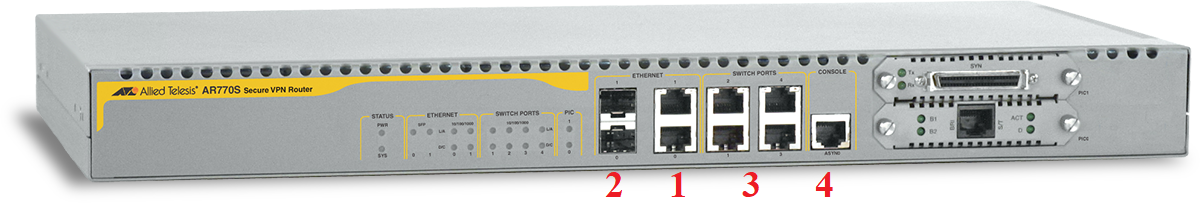
\includegraphics[width=\linewidth]{ar770s}
%	\caption{Ο δρομολογητής Allied Telesis AR770S}\label{fig:ar770s}
%\end{figure}
%Οι δρομολογητές Allied Telesis AR770S αποτελούνται από τις εξής διεπαφές:
%\begin{enumerate}
%	\item x2 θύρες Gigabit Ethernet (WAN)
%	\item x2 θύρες SFP (WAN)
%	\item x4 θύρες Gigabit Ethernet (switch ports - LAN)
%	\item x1 Θύρα κονσόλας RJ-45
%	\item x2 υποδοχές για κάρτες επέκτασης
%\end{enumerate} 

%Οι δρομολογητές Allied Telesis AR770S εκτελούν όλες τις λειτουργίες ενός συμβατικού δρομολογητή, με τη διαφορά ότι είναι ειδικά σχεδιασμένοι σε επίπεδο υλικού ώστε να υποστηρίζουν με υψηλές επιδόσεις υπηρεσίες VPN, ταυτόχρονα με NAT, καταστατική επιθεώρηση πακέτων (stateful packet filtering - SPI) και ποιότητα υπηρεσιών (QoS), λειτουργίες απαιτητικές σε επεξεργαστική ισχύ και μνήμη.

%Λειτουργικό σύστημα των δρομολογητών Allied Telesis είναι το AlliedWare OS. Το συγκεκριμένο λειτουργικό σύστημα έχει, πλέον, εγκαταλειφθεί και έχει αντικατασταθεί από το AlliedWare Plus, το οποίο είναι σχεδόν ίδιο με το Cisco IOS. 

\end{document}
